%%% Fiktivní kapitola s ukázkami sazby

\chapter{Analýza požadavků}

Kapitola analýza požadavků se věnuje první fázi ve vývoji softwarového projektu. Analýza požadavků se skládá z různých fází dle použité metodiky, ale vždy je cílem od relevantních stran získat seznam požadavků, co aplikace musí splňovat, aby naplnila cíle, kvůli kterým se k vývoji SW projektu rozhodlo. V jiných slovech je tedy část analýzy požadavků kritická pro úspěch softwarového projektu \cite{maguire2002user}.

% chce to zdroje, a ten text je taky dost divný

\section{Identifikace stakeholderů}

% vysvětlit pojem stakeholder, jak se dělá analýza stakeholderů

Identifikace stakeholderů je první fází v analýze požadavků. Účelem této fáze je identifikovat všechny relevantní zúčastněné strany, aby mohly být zapojeny do fáze sběru požadavků a přiřadit k nim jednotlivé případy užití aplikace \cite{maguire2002user}. V případě nedostatečného zapojení stakeholderů je vysoká pravděpodobnost, že software nebude uspokojovat potřeby všech zúčastněných stran.

Za stakeholdery byly identifikovány následující subjekty: stávající uživatele webové aplikace Anitra a majitel firmy Anitra System s.r.o.

Stávající uživatelé aplikace již požadovali funkce pro práci v terénu a jejich požadavky byly zaevidovány do pořadníku funkcí pro webovou aplikaci. Tyto požadavky byly konzultovány se zakladatelem firmy Anitra a byly vybrány k řešení. Zakladatel firmy je projektovým manažerem a komunikuje se zákazníky na denní bázi, má tedy dostatečný přehled o požadavcích zákazníků a jejich priorit, zároveň působí i jako kontaktní bod podpory pro aplikaci. Cílem zakladatele firmy je poskytnout uživatelům nástroje pro efektivní práci v terénu i pro rychlou kontrolu dat z mobilních zařízení, což by mohlo být bráno jako konkurenční výhoda, jelikož na trhu nebyla nalezena podobná aplikace.

\section{Sběr požadavků}

Pro zakladatele firmy Anitra je cílem mobilní aplikace doplnění ekosystému značky Anitra o vhodné řešení zobrazení a zadávání dat v terénu. Na začátku práce byla pouze dostupná webová aplikace, která měla pro práci v terénu následující nevýhody:

\begin{itemize}
	\item data po odpojení z internetu nebyla dostupná, ve většině případů ani již načtená data,
	\item aplikace byla příliš náročná na energii,
	\item mapové podklady se nezobrazovaly po odpojení ze sítě,
	\item aplikace byla na datový přenos příliš náročná,
	\item navigace v GUI byla pro malá zařízení příliš složitá.
\end{itemize}

Tyto podněty byly sebrány od uživatelů webové aplikace Anitra v období 2018-2020, ale mělo by se jednat o dostatečný základ pro zařazení mobilní aplikace do portfolia ekosystému Anitra, jelikož se jedná o obecné předpoklady pro software tohoto typu.

Z těchto zkušeností uživatelů vyplynuly klíčové funkční i nefunkční požadavky na funkcionalitu aplikace. Jednotlivé části jsou rozebrány níže. Další funkční požadavky byly definovány zakladatelem firmy Anitra (zde uvedeny ve zkrácené formě, seřazeny dle priority):

\begin{itemize}
	\item zobrazit poslední polohu zařízení v mapě,
	\item možnost stáhnout si mapy před kontrolou na místě,
	\item zobrazení dat ze zařízení,
	\item zobrazení vlastní pozice na mapě
	\item notifikace o nových datech,
	\item zaznamenat trasu, bod,
	\item možnost přiložit obrázek k zvířeti.
\end{itemize}

\section{Funkční požadavky}

Funkční požadavky popisují očekávané chování systému, ale nevěnují se technickým detailům, jak má systém fungovat. Funkční požadavky slouží pro splnění potřeby uživatelů a lze je vyjádřit ve formě případů užití nebo diagramu případu užití \cite{jacobson1987object}.

Jednotlivé případy užití jsou rozebrány v kapitole uvedené níže.

\subsection{Diagram případů užití}

Diagram případu užití je diagramem ze standardní sady UML využívané v softwarovém inženýrství.

\begin{figure}[H]
	\begin{center}
		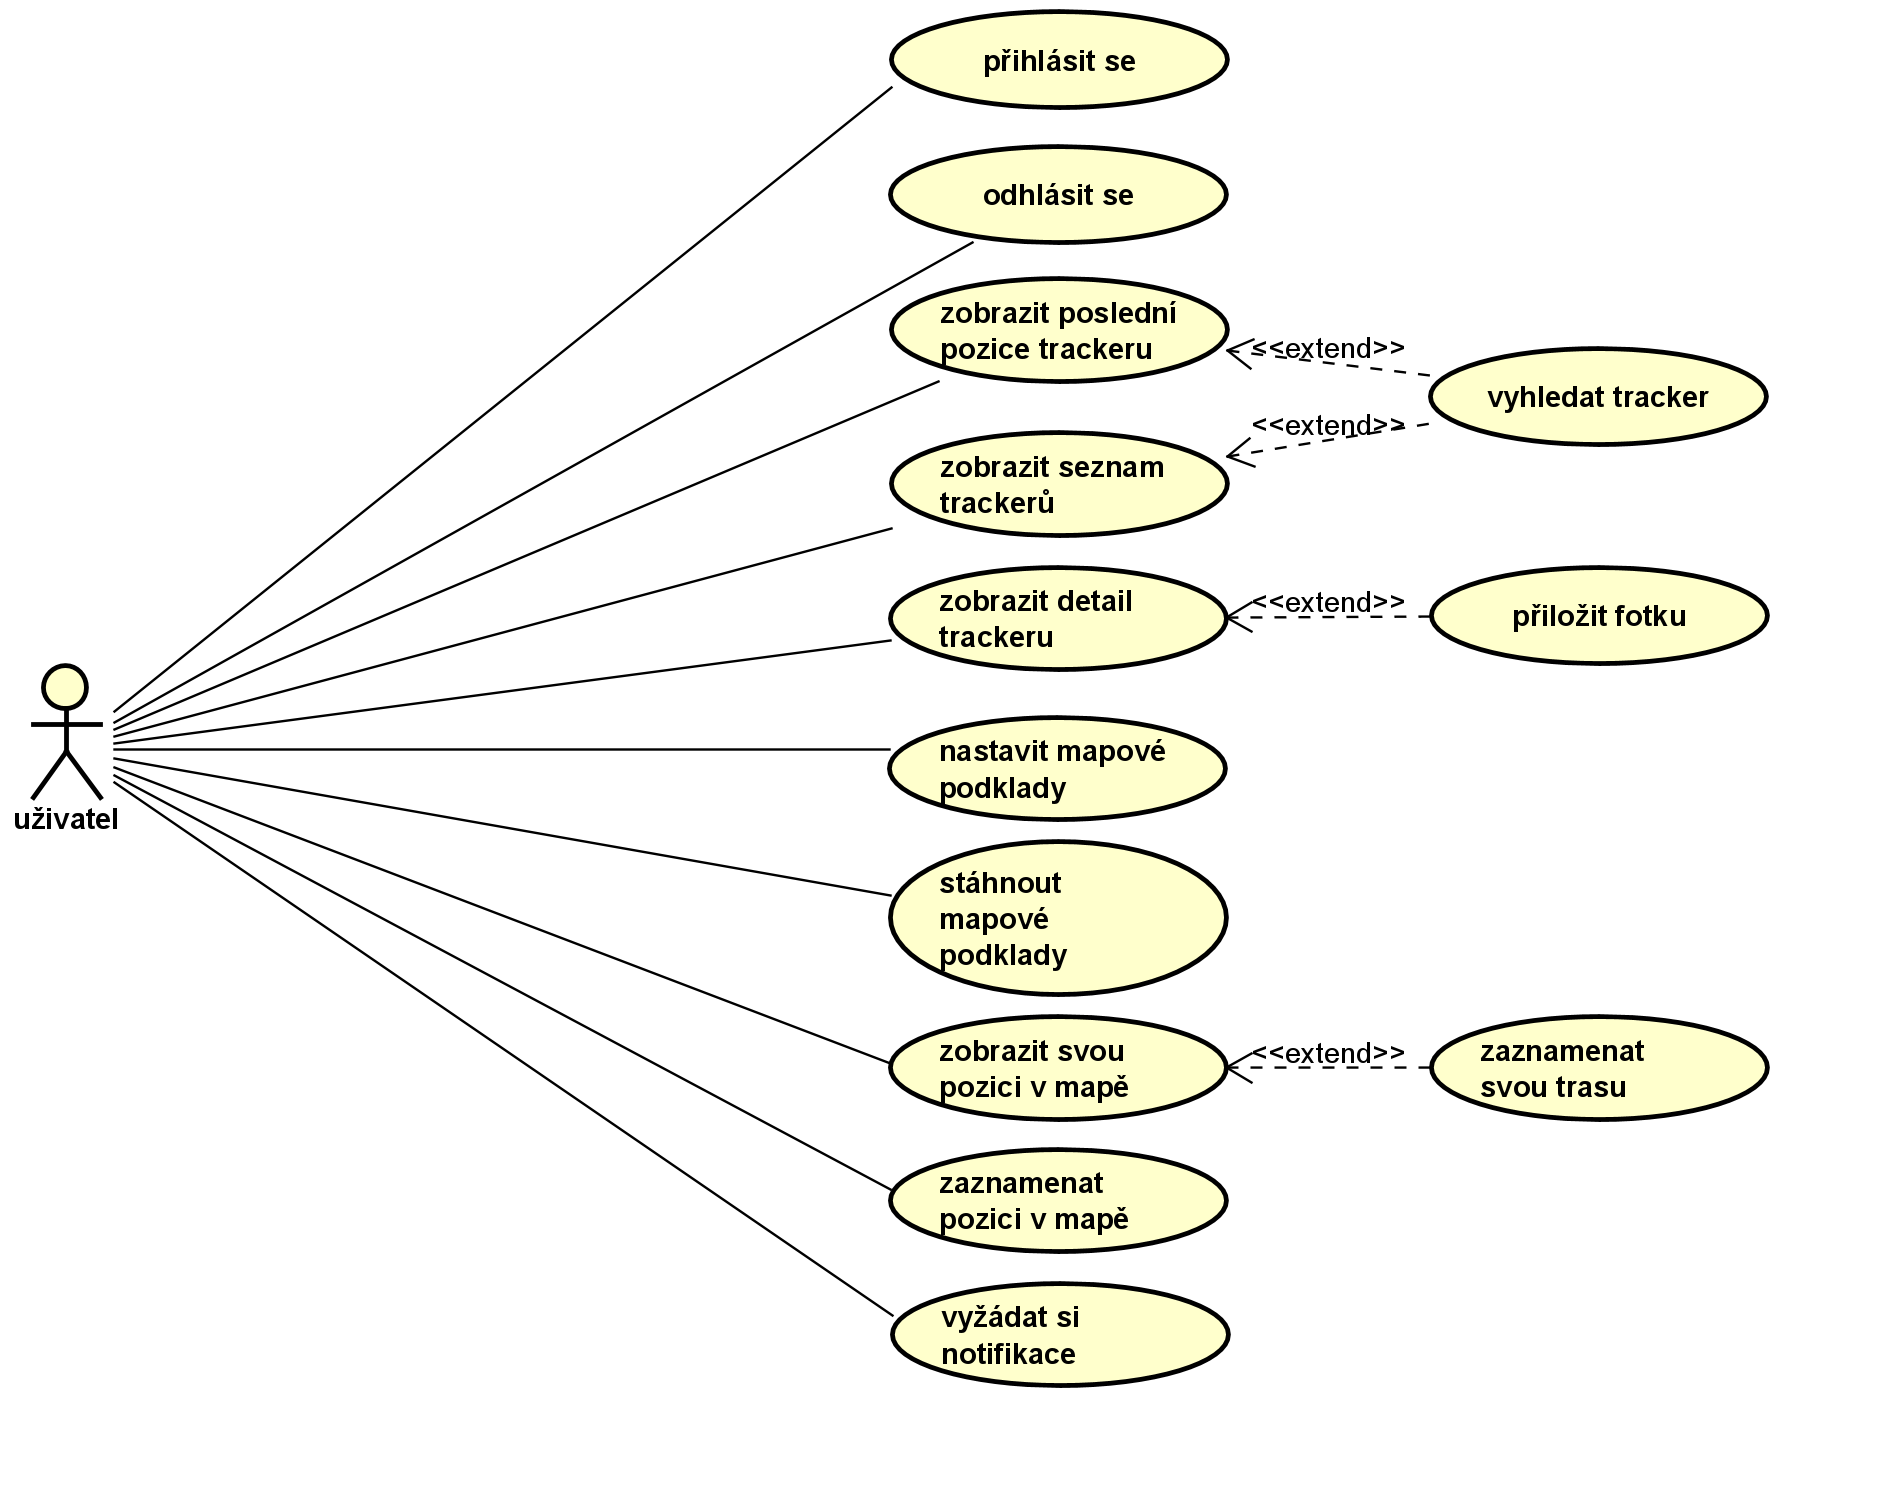
\includegraphics[width=140mm]{img/usecase.png}
	\end{center}
	\caption[Diagram případu užití]{Diagram případu užití -- zdroj: autor}
\end{figure}

Diagram případů užití byl sestaven dle nasbíraných požadavků zmíněných v minulé kapitole. Případy užití byly rozšířeny o nevyslovené, ale odvoditelné požadavky, např. možnost přihlásit se a odhlásit se.

\section{Nefunkční požadavky}

Nefunkční požadavky udávají kvalitu systému, ale ne jeho chování. Tyto požadavky často přináší omezení do implementací funkčních požadavků a je někdy obtížné tyto požadavky sladit, mohou působit i protichůdně. Jako příklad se často uvádí požadavky spojené s komfortem uživatelů (např. přístupnost, výkonnost, lokalizace), provozem aplikace (přenositelnost, tolerance chyb) a bezpečnost. Do nefunkčních požadavků se řadí i požadavky související s možností dalšího vývoje systému \cite{chung2012non}.

Z výše uvedeného seznamu požadavků vyplynulo několik klíčových nefunkčních požadavků především ve vztahu k uživatelům. Pro úspěch aplikace je nutné, aby grafické rozhraní aplikace bylo dostatečně jednoduché a podstatné funkce byly rychle přístupné bez složitých navigací, jelikož uživatel nemusí mít mnoho času pro práci s aplikací v terénu. S tímto souvisí i nutnost odezvy v jednotkách sekund. 

Neuvedeným požadavkem je multiplatformnost aplikace, jelikož část uživatelů stávající aplikace využívá mobilní operační systém iOS a část Android. Podstatným požadavkem je i rozšiřitelnost aplikace, jelikož se s vývojem aplikace počítá i po dokončení této práce.

\section{Časové aspekty}

Aplikace má být vyvinuta a nasazena nejpozději do konce května, ideálně již v dubnu. V tuto dobu probíhá nejvyšší počet ornitologických operací spojených s nasazováním trackerů, kontrolou hnízd a dalších. Aplikaci nebylo možné začít vyvíjet dříve než v polovině února kvůli návaznosti na API již existující webové aplikace. Pro prvotní verzi aplikace je kritické aby spolehlivě zobrazovala poslední body v mapě a po prvotní synchronizaci fungovala bez internetového připojení.
